\documentclass[tikz,border=10pt]{standalone}

\usepackage[T1]{fontenc}
\usepackage[utf8]{inputenc}
\usepackage{lmodern}
\usetikzlibrary{arrows.meta,positioning}

\definecolor{oink}{HTML}{253238}
\definecolor{omuted}{HTML}{647178}
\definecolor{oaccent}{HTML}{9FA8AC}
\definecolor{osoft}{HTML}{F1F2F2}

\begin{document}
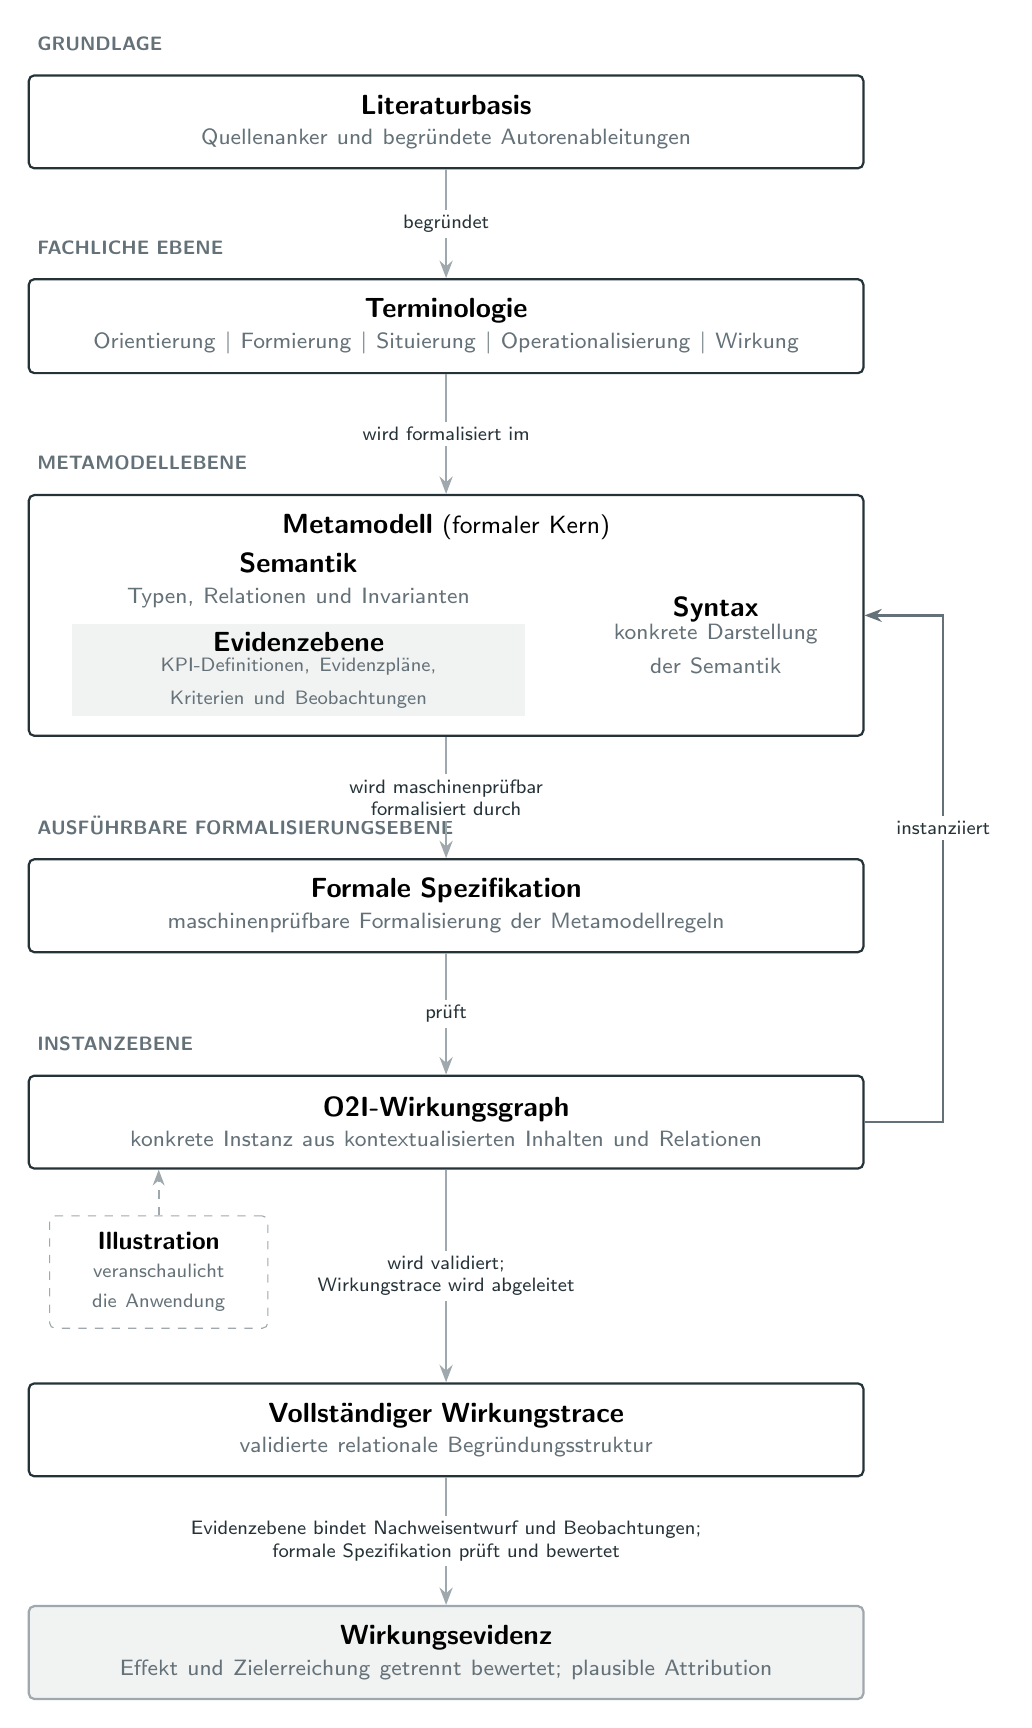
\begin{tikzpicture}[
  box/.style={
    draw=oink,
    fill=white,
    line width=0.8pt,
    rounded corners=2pt,
    minimum width=10.6cm,
    minimum height=1.18cm,
    text width=9.9cm,
    align=center,
    inner sep=7pt,
    font=\sffamily
  },
  result/.style={box, draw=oaccent, fill=osoft},
  supporting/.style={
    draw=oaccent,
    fill=white,
    dashed,
    rounded corners=2pt,
    text width=2.35cm,
    align=center,
    inner sep=6pt,
    font=\sffamily\small
  },
  flow/.style={-{Stealth[length=2.2mm]}, draw=oaccent, line width=1pt},
  return flow/.style={-{Stealth[length=2.2mm]}, draw=omuted, line width=0.85pt},
  support flow/.style={-{Stealth[length=2mm]}, draw=oaccent, dashed, line width=0.85pt},
  relation/.style={
    fill=white,
    align=center,
    inner xsep=5pt,
    inner ysep=2pt,
    text=oink,
    font=\sffamily\scriptsize
  },
  level/.style={font=\sffamily\scriptsize\bfseries, text=omuted}
]

\node[box] (literature) {
  \textbf{Literaturbasis}\\[-1pt]
  {\footnotesize\color{omuted}Quellenanker und begründete Autorenableitungen}
};
\node[level, anchor=south west] at ([yshift=0.18cm]literature.north west) {GRUNDLAGE};

\node[box, below=1.38cm of literature] (terminology) {
  \textbf{Terminologie}\\[-1pt]
  {\footnotesize\color{omuted}Orientierung \textbar{} Formierung \textbar{} Situierung
  \textbar{} Operationalisierung \textbar{} Wirkung}
};
\node[level, anchor=south west] at ([yshift=0.18cm]terminology.north west) {FACHLICHE EBENE};

\draw[flow] (literature) -- node[relation] {begründet} (terminology);

\node[box, below=1.52cm of terminology, minimum height=2.78cm] (metamodel) {
  \textbf{Metamodell} {\small(formaler Kern)}\\[4pt]
  \begin{minipage}{6.15cm}
    \centering
    \textbf{Semantik}\\[-1pt]
    {\footnotesize\color{omuted}Typen, Relationen und Invarianten}\\[5pt]
    \colorbox{osoft}{\parbox{5.55cm}{\centering
      \textbf{Evidenzebene}\\[-1pt]
      {\scriptsize\color{omuted}KPI-Definitionen, Evidenzpläne,\\
      Kriterien und Beobachtungen}}}
  \end{minipage}
  \hfill
  \begin{minipage}{3.05cm}
    \centering
    \textbf{Syntax}\\[-1pt]
    {\footnotesize\color{omuted}konkrete Darstellung\\der Semantik}
  \end{minipage}
};
\node[level, anchor=south west] at ([yshift=0.18cm]metamodel.north west) {METAMODELLEBENE};

\draw[flow] (terminology) -- node[relation] {wird formalisiert im} (metamodel);

\node[box, below=1.54cm of metamodel] (specification) {
  \textbf{Formale Spezifikation}\\[-1pt]
  {\footnotesize\color{omuted}maschinenprüfbare Formalisierung der Metamodellregeln}
};
\node[level, anchor=south west] at ([yshift=0.18cm]specification.north west) {AUSFÜHRBARE FORMALISIERUNGSEBENE};

\draw[flow] (metamodel) -- node[relation] {
  wird maschinenprüfbar\\formalisiert durch
} (specification);

\node[box, below=1.54cm of specification] (graph) {
  \textbf{O2I-Wirkungsgraph}\\[-1pt]
  {\footnotesize\color{omuted}konkrete Instanz aus kontextualisierten Inhalten und Relationen}
};
\node[level, anchor=south west] at ([yshift=0.18cm]graph.north west) {INSTANZEBENE};

\draw[flow] (specification) -- node[relation] {prüft} (graph);
\draw[return flow]
  (graph.east) -- ++(1.0,0) |- node[relation, pos=0.29] {instanziiert} (metamodel.east);

\node[supporting, anchor=north] at ([xshift=-3.65cm,yshift=-0.58cm]graph.south) (illustration) {
  \textbf{Illustration}\\[-1pt]
  {\scriptsize\color{omuted}veranschaulicht die Anwendung}
};
\draw[support flow] (illustration.north) -- ([xshift=-3.65cm]graph.south);

\node[box, below=2.70cm of graph] (trace) {
  \textbf{Vollständiger Wirkungstrace}\\[-1pt]
  {\footnotesize\color{omuted}validierte relationale Begründungsstruktur}
};

\draw[flow] (graph) -- node[relation] {
  wird validiert;\\Wirkungstrace wird abgeleitet
} (trace);

\node[result, below=1.62cm of trace] (evidence) {
  \textbf{Wirkungsevidenz}\\[-1pt]
  {\footnotesize\color{omuted}Effekt und Zielerreichung getrennt bewertet; plausible Attribution}
};

\draw[flow] (trace) -- node[relation] {
  Evidenzebene bindet Nachweisentwurf und Beobachtungen;\\
  formale Spezifikation prüft und bewertet
} (evidence);

\end{tikzpicture}
\end{document}
